\documentclass[12pt,twocolumn,letterpaper]{article}
\usepackage[a4paper,top=2.54cm,bottom=2.54cm,left=2cm,right=2cm,marginparwidth=1.75cm]{geometry}
\usepackage[english, chinese]{babel}
\usepackage[utf8x]{inputenc}
\usepackage[T1]{fontenc}
\usepackage{xeCJK}
\setCJKmainfont{Noto Serif CJK TC}
\usepackage{setspace}
\onehalfspacing
\usepackage{amsmath}
\usepackage{graphicx}
\usepackage[colorinlistoftodos]{todonotes}
\usepackage[colorlinks=true,urlcolor=black, linkcolor=red,citecolor=blue]{hyperref}
\usepackage{authblk}
\usepackage[square,numbers]{natbib}
\bibliographystyle{unsrt}
%\usepackage{cite}
\usepackage[capitalize]{cleveref}
\usepackage[numbered]{bookmark}
\usepackage{ntheorem}
\newtheorem{hyp}{假設} 

\newtheorem{theorem}{Theorem}
\newtheorem{corollary}{推論}
\newtheorem{explain}{解釋}

%%%%%%%%%%%%%%%%%%%%%%%%%%%%%%%%%%%%%%%%%%%%%%%%%%%
\crefname{table}{表}{表}  
%\Crefname{table}{表}{表}
\crefname{figure}{圖}{圖}  
%\Crefname{figure}{圖}{圖}
\crefname{corollary}{推論}{推論}
\crefname{hyp}{假設}{假設}
\crefname{section}{段落}{段落}
\addto{\captionsenglish}{\renewcommand{\abstractname}{摘要}}
\addto{\captionsenglish}{\renewcommand{\figurename}{圖}}
\addto{\captionsenglish}{\renewcommand{\tablename}{表}}

%%%%%%%%%%%%%%%%%%%%%%%%%%%%%%%%%%%%%%%%%%%%%%%%%%%
\providecommand{\keywords}[1]
{
  \small	
  \textbf{\textit{Keywords---}} #1
}

%%%%%%%%%%%%%%%%%%%%%%%%%%%%%%%%%%%%%%%%%%%%%%%%%%%
% Title
\title{
		\LARGE\bf 
		基於社交媒體的政治情感分析:
		美媒於總統選舉前後對中態度調查 \\
}

% Author
\author[$\dagger$]{呂宣誼(\texttt{B07303084})}
\author[$\dagger\ddagger$]{邱威諭(\texttt{B07303037})}
\author[$\dagger$]{楊尚霖(\texttt{B07303116})}
\author[$\dagger$]{\\赫謙(\texttt{B07303118})}
\author[$\ddagger$]{郭宇杰(\texttt{B07611039})}
\affil[$\dagger$]{台大經濟系}
\affil[$\ddagger$]{台大資管系}

\date{\vspace{-5ex}}

%%%%%%%%%%%%%%%%%%%%%%%%%%%%%%%%%%%%%%%%%%%%%%%%%%%
% Renewcommand
\renewcommand{\bibsection}{\section*{參考資料}}

%%%%%%%%%%%%%%%%%%%%%%%%%%%%%%%%%%%%%%%%%%%%%%%%%%%
\begin{document}
\maketitle

\begin{abstract}
    本文爬梳了美國媒體於推特上與中國
    有關的報導,
    並分析於選舉前後媒體對待中國的態度
    是否有所差異。
    實驗結果顯示,選舉前後媒體報導對
    中國態度有所差異,
    且各間媒體呈現相似的趨勢:選後對
    中國的態度較為平緩;
    選舉前後媒體所報導
    與中國有關的主題也不盡相同,
    如選舉前「香港」是常見的報導主題,
    選後則較少出現於報導中,
    而「台灣」則較常見於選後的報導。
\end{abstract}

\keywords{美中關係、隱藏語意分析、情感分析、社群媒體分析}

% 由於我們認為美國媒體在總統競選前後對於中國的報導主題、風向與態度可能會有差異,因此我們利用推特平台搜集不同立場傾向的媒體


\section{專案動機}\label{sec:motiv}
美國與中國已然是當今世界上最強勢的兩大國家,
兩大強權之間的關係皆是各國矚目的焦點。
自二十世紀開始,中美之間的關係從戰爭同盟國、從支持中華民國政府轉為
與中華人民共和國政府建交,到現今彼此防範彼此,
美中關係的變化受到其領導人的風格與國家路線影響甚鉅,
媒體的態度能於一定程度上反映出國家對於某項
議題的想法與關注度,尤其是針對政治議題,
例如當局政府相當親中時,
媒體可能就會傾向於報導美中關係的建立;
若當局政府相當厭中,
則媒體可能會產出較多兩國衝突的報導。
在資訊產生及傳播相當快速的當代社會,
資訊往往係透過媒體的反芻消化後才進到閱聽人
的眼裡耳中,媒體對待某個議題的態度對於資訊便顯得十分重要。
因此我們好奇,美國媒體在選舉前後,
面對兩個對待中國態度截然不同的候選人與政府,
針對中國的態度是否會有所不同。

本文的架構如下:
\cref{sec:LR} 爬梳了社交媒體與政治情感分析領的相關研究;
\cref{sec:struc} 介紹我們如何設定資料範圍、
資料爬取方法、資料的前處理;
\cref{sec:exp} 整理了我們所做的研究與實驗,
包含研究方法、實驗結果等。
\cref{sec:conclu} 在文末總結這份研究。


\section{文獻回顧}\label{sec:LR}
針對社群媒體與情感分析有許多的研究和文獻著墨於上,
例如最早\cite{twt}首次使用Twitter平台進行政治情感分析,
並發現Twitter確實可以用來反映選舉結果,
進而預測選舉。
隨著機器學習技術的革新以及計算資源的突破,有更多的方法能夠使用在這類型的分析上。
\cite{svm}設計了一種結合Twitter流量和情感分析的模型進行選舉結果預測,
並使用文檔中的單詞作為向量,
訓練支持向量機(Support Vector Machine, SVM)分類器對文本進行情感分析;
\cite{RNN}採用遞歸神經網路(Recurrent Neural Networks, RNN)
與長短期記憶模型(Long Short-Term Memory, LSTM)的方法
進行政治情感分析與分類;
而\cite{embed}則將詞嵌入(Word Embeddings)融合卷積神經網路
(Convolution Neural Networks)對
Twitter的資料進行選舉預測分類。
多數政治情感分析的研究都是著墨於選舉結果,
\cite{emo}的研究則是揭露了
政治傾向、正負字詞與候選人間的關聯性認知影響,啟發了我們的研究方向。
除了分析方法的不同外,\cite{press}分析了美國的政治光譜與主流媒體的傾向,\cite{RRPFI}調查美國民眾對中的好感度,
我們也參考\cite{press, RRPFI}所得出的結果分析美國媒體的對中態度。

\section{資料蒐集與評估}\label{sec:struc}
\subsection{資料蒐集}
為了預估民眾態度可能會轉變的時間點,我們首先整理西元2019至2021年
之間發生的中美事件,如2020年3月2號時,
美國國務院宣布將對五家中國官方媒體機構實施雇員;
2021年2月11日時拜登上任總統後首次和中國國家主席習近平通話等。
基於上述時間段,我們將關鍵字設為「China」,
抓取2020年至2021年(美國總統大選前後各10個月)
美國人主流新聞媒體推特上的推文,
最後選定ABC、NBCnews、CNN、CBSNews、nytimes、
WSJ、FoxNews七間媒體進行分析。

\subsection{資料前處理}
我們使用推特開放的高級搜索API\footnote{\url{https://twitter.com/search-advanced}}
訪問目標推特帳號的貼文
並抓取目標媒體的帳號ID、推文內容、日期與網址。
我們將資料的不同欄位進行若干前處理,如將API爬下來後的預設日期
轉為格式化日期、
推文內容去除對分析沒有用的標點符號(如[*]\$@~\%+=)等等。

\section{實驗設計}\label{sec:exp}
我們首先根據\cite{RRPFI} 的結果針對資料進行假設:

\begin{hyp}\label{hyp:attitude}
美國媒體於選前選後的對中態度會有所差異。
\end{hyp}
\begin{hyp}\label{hyp:topic}
美國媒體於選前選後關注的對中議題並不相同。
\end{hyp}

另外,我們也想知道我們分析出來的媒體
態度是否符合\cite{press} 的調查,
因此我們設定了另一個假設:
\begin{hyp}\label{hyp:press}
各家不同立場之媒體的報導風格與主題皆不同。
\end{hyp}

基於這三個假設,我們設計了一系列的實驗
來分析資料是否符合我們的假設。

\subsection{對中態度的情感分析}\label{subsec:sent}
\subsubsection{模型與套件}
挑選適合的模型與套件對於資料分析而言是相當重要
的前置作業。我們分析TextBlob\footnote{\url{https://textblob.readthedocs.io/en/dev/}}、flair\footnote{\url{https://github.com/flairNLP/flair}}、twitter-roberta-base-sentiment\footnote{\url{https://huggingface.co/cardiffnlp/twitter-roberta-base-sentiment}}三個常用的情感分析套件,
發現TextBlob太過粗糙,將不在語料庫內的字都視為
沒有情感;flair又太過敏感,結果幾乎都是落在光譜的
兩端,最後我們選定使用支援表情符號,
且將表情符號納入分析語料中的twitter-roberta-base-sentiment套件。而處理Word Embeddings的工具,我們則是
使用較為靈敏與準確的bert-base-multilingual-uncased-sentiment\footnote{\url{https://huggingface.co/nlptown/bert-base-multilingual-uncased-sentiment}},而非上課提及的Keras BERT\footnote{\url{https://github.com/CyberZHG/keras-bert}}。

\subsubsection{統計圖表與討論}
透過圖表反應資料趨勢是常見的資料視覺化手法,
我們製作不同媒體報導資料的情感分數與頻率之間的
直方圖,取NBCNews的結果為例,
呈現如\cref{fig:hist}。
其中上半部是選舉前的頻率分佈直方圖,
下半部則是選舉後的頻率分佈直方圖。
\begin{figure}[h!]
    \centering
    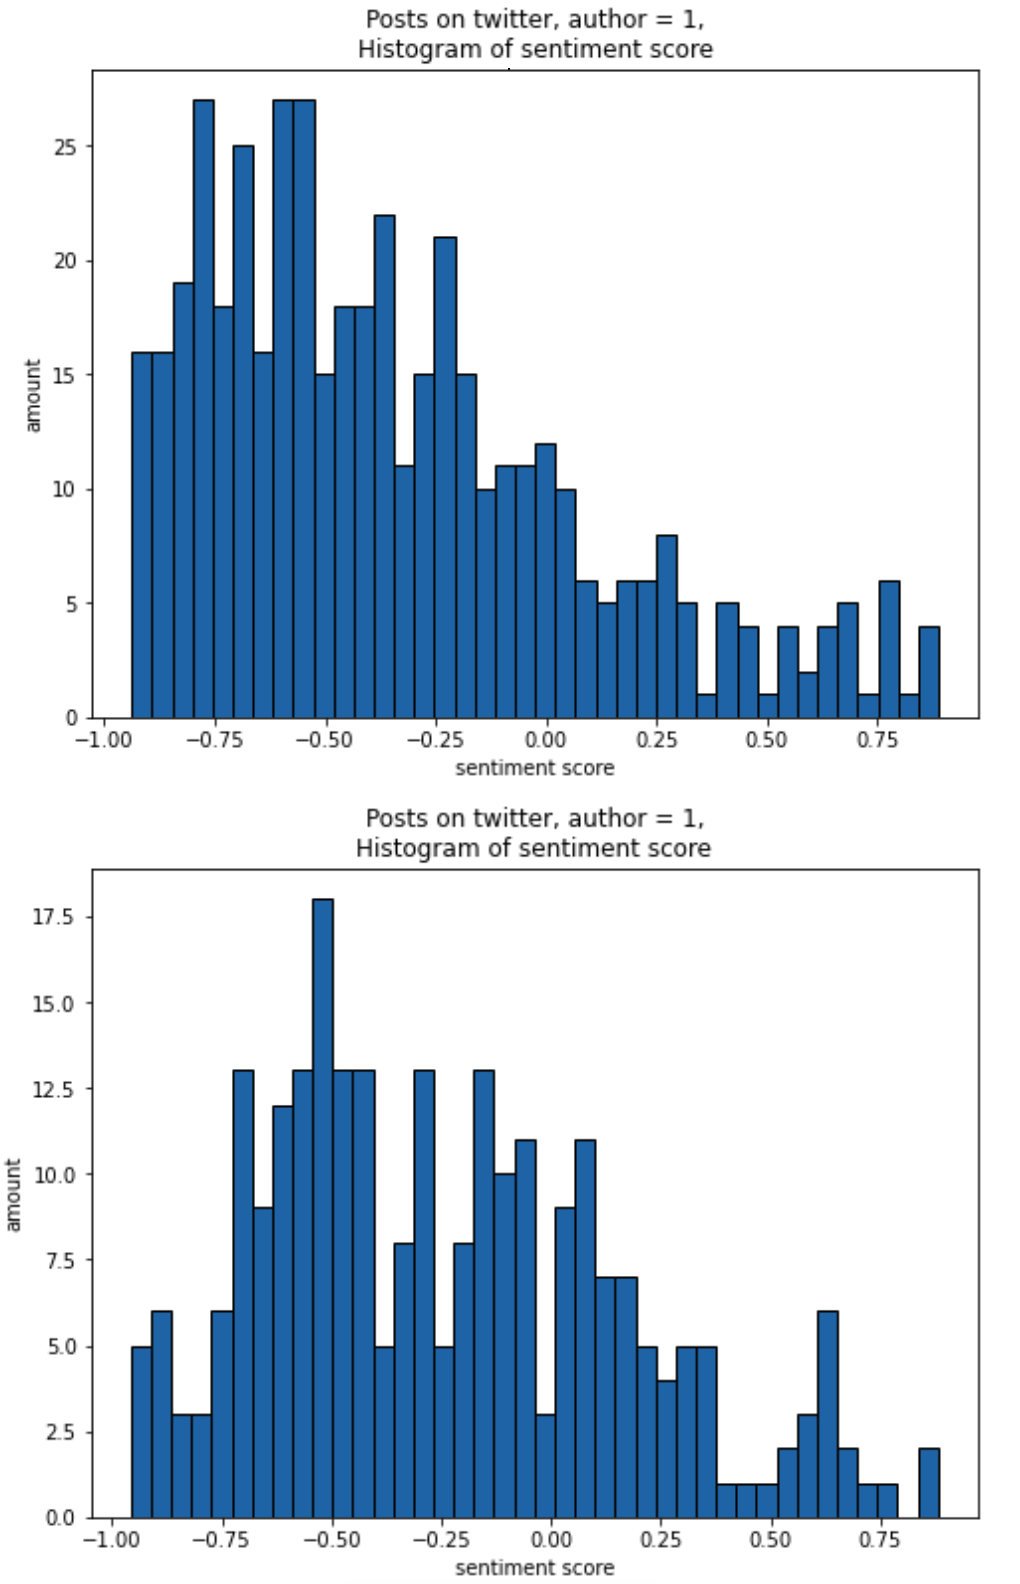
\includegraphics[width=0.8\linewidth]{Figure/histogram.png}
    \caption{NBCNews情感分數頻率的直方圖}
    \label{fig:hist}
\end{figure}


\begin{figure*}[htp!]
    \centering
    \begin{minipage}{0.9\textwidth}
    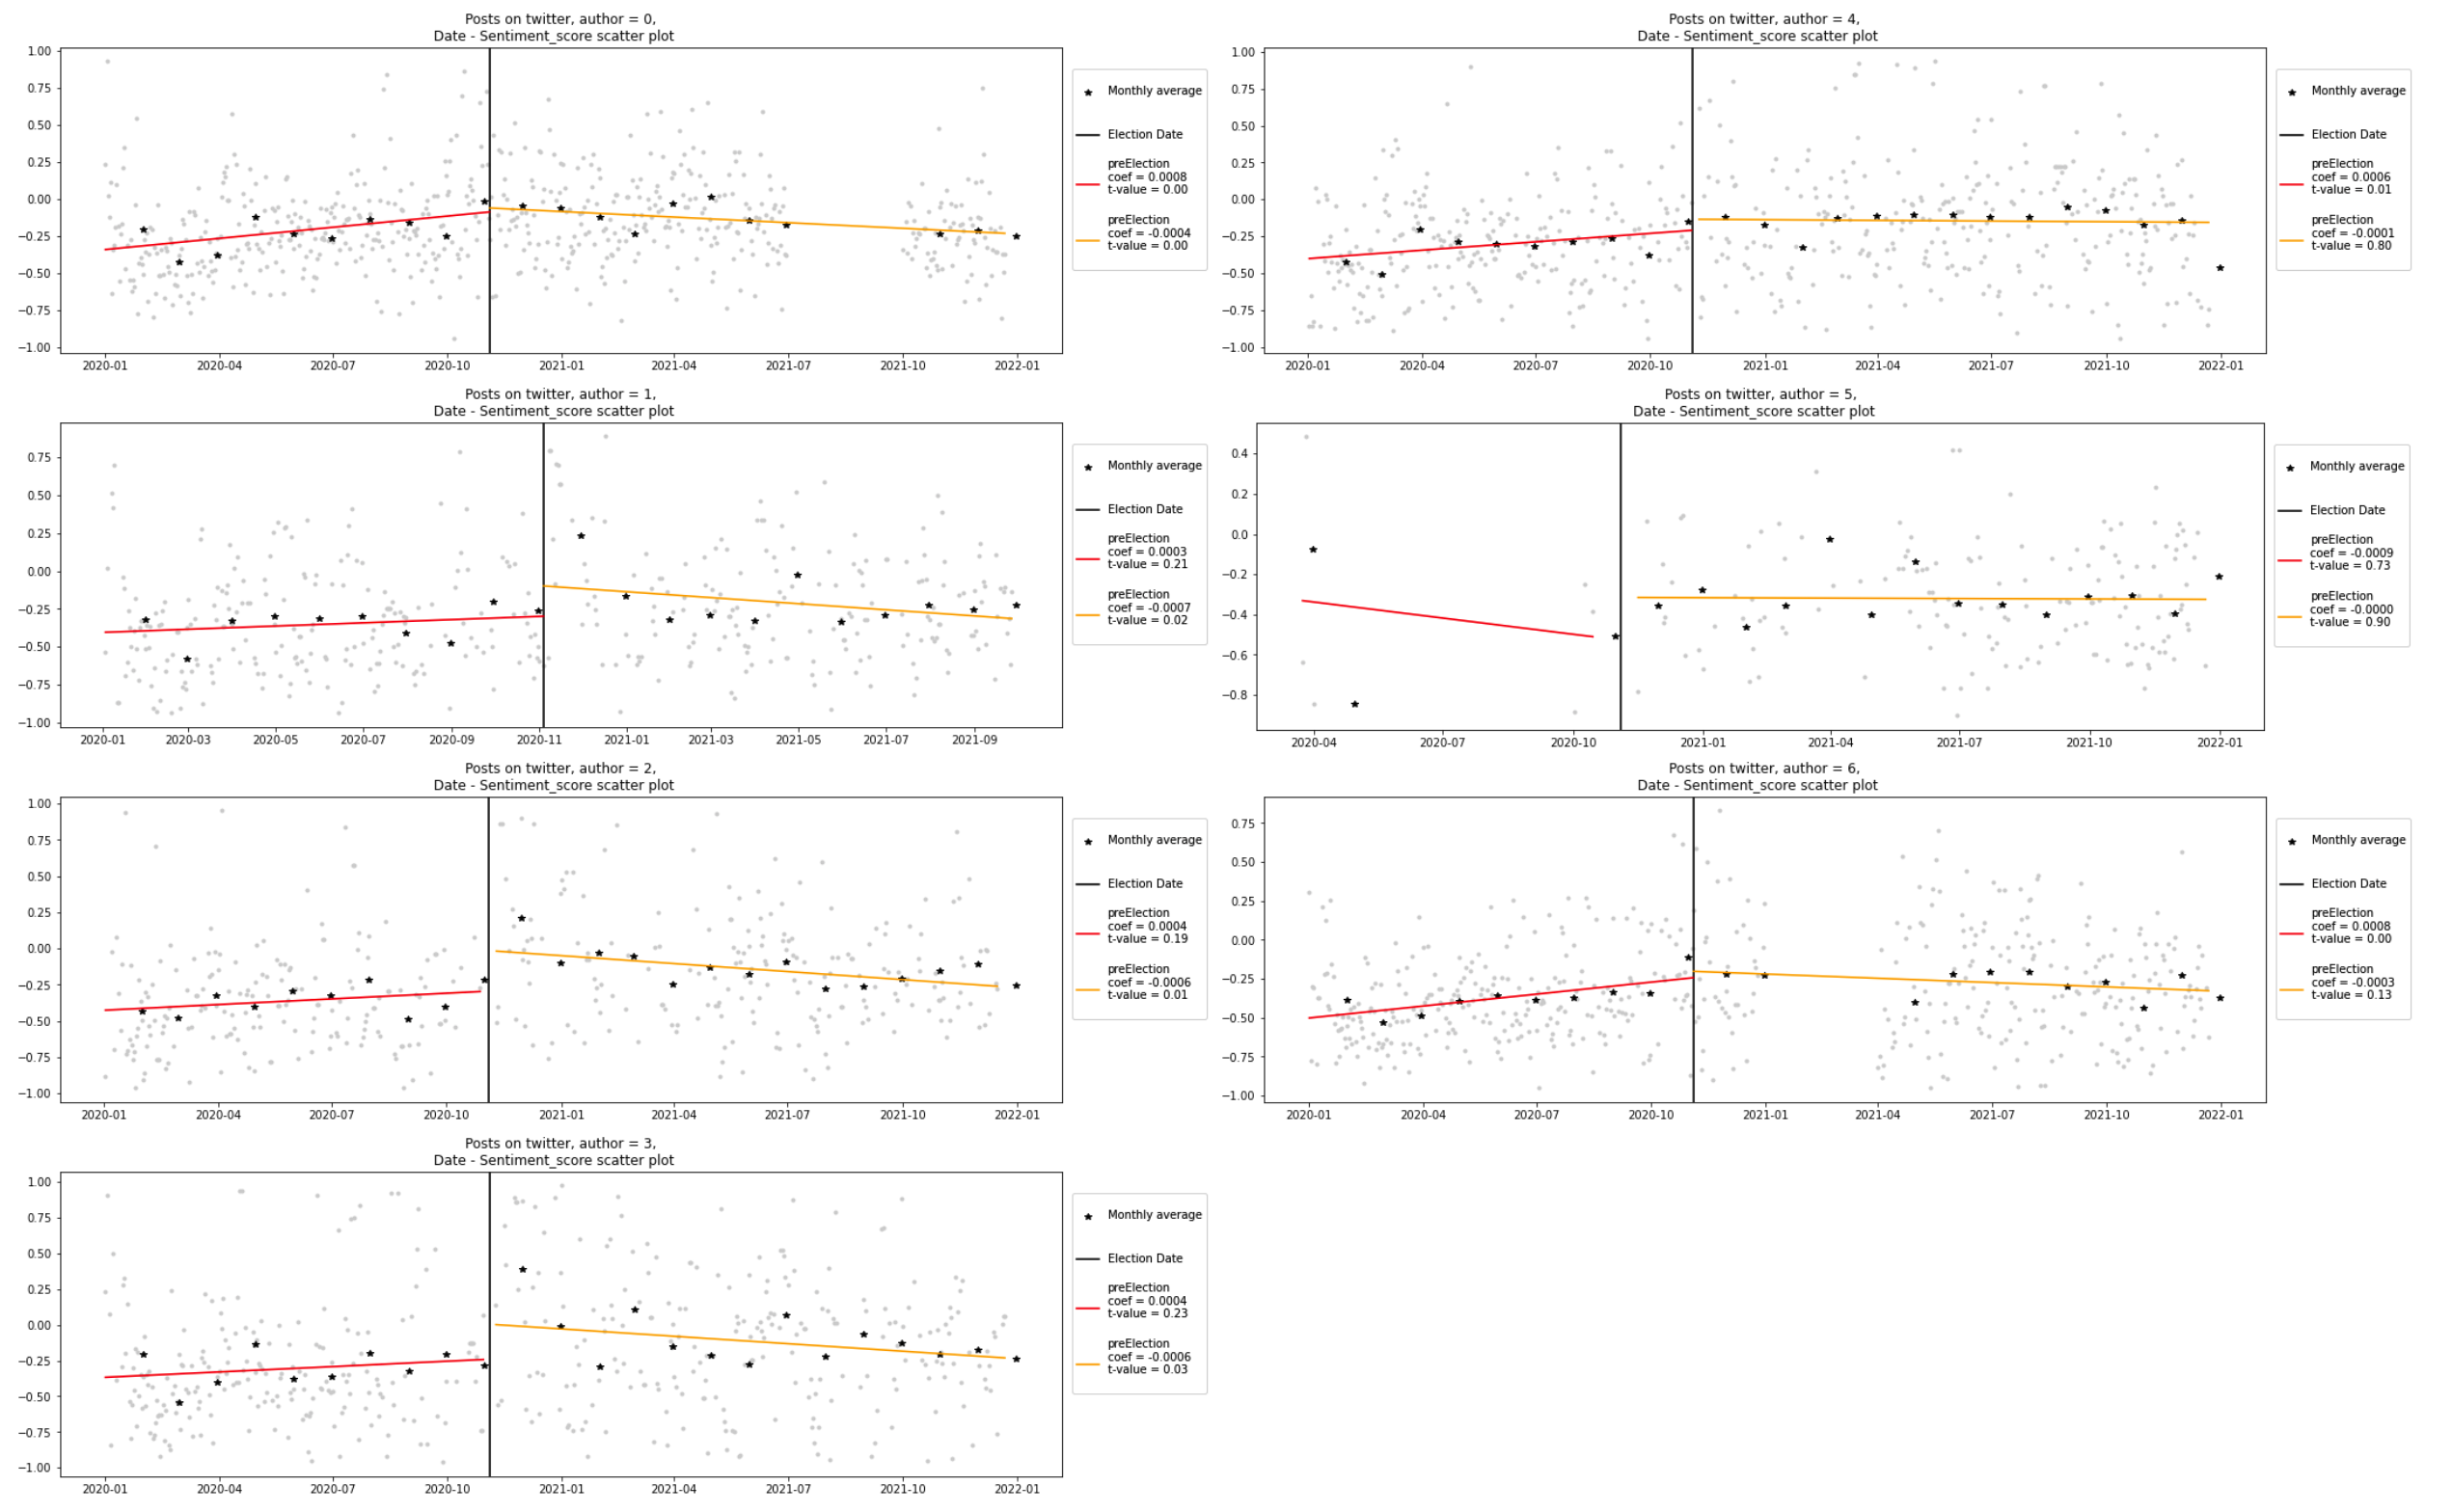
\includegraphics[width=\linewidth]{Figure/scatter.png}
    {\footnotesize 
    此圖為時間自2020至2021年間各間
    媒體推文報導的情感分數散佈圖,
    以黑線標示美國總統選舉日期,
    黑線以左代表選舉前,
    以右則為選舉後。
    紅線代表選舉前的推文報導情感分數
    趨勢,
    黃線則代表選舉後的推文報導情感分數
    趨勢。
    \par}
    \end{minipage}
    \caption{報導推文情感分數之時間序列點狀圖}
    \label{fig:scatter}
\end{figure*}

由於七間媒體選前選後的情感分數頻率趨勢相似,
選前情感分數低的推文頻率較高、
選後則分布較為平均,
因此我們有以下推論:



\begin{corollary}\label{cor:attr}
選舉前後媒體對中態度有影響,
且選後態度較為中立。
\end{corollary}

緊接著,我們也製作了隨著時間推進,
不同媒體報導推文情感分數的點狀圖,如
\cref{fig:scatter} 。
\cref{fig:scatter} 的T-value
揭示了結果的顯著性,而根據
其選舉前後的情感分數趨勢
也論證了\cref{cor:attr} 。
而針對這般結果,我們試圖給予合理的解釋。
\begin{explain}\label{exp:attr}
我們認為,由於民眾普遍不喜歡總統候選人川普
,因此並不會特別關注其所支持的反中相關議題。
且2020與2021年間適逢疫情,
選舉期間所關注的中國議題應有部分
是醫療相關。
\end{explain}

\subsection{不同媒體的報導風格與對中態度}\label{subsec:style}
選舉前後媒體對中態度是否不同,
\cref{subsec:sent} 
已經給出了肯定的答案,
而我們接著想繼續探討選舉前後,
不同媒體的報導主題是否一致,且是否如
\cref{hyp:press} 所述,
不同立場媒體間的風格與主題會有所不同。
我們採用分群演算法的方式,
企圖將所有的報導依據媒體、對中態度等分到不同的群集,惟效果非常不好,
幾乎所有的資料都被分到同一個群集中。
\begin{explain}\label{exp:bias}
由於蒐集到的資料本身就有偏誤,
資料本身過於相似,
分群演算法很容易將所有資料直接視為同一群。
\end{explain}


仔細思考後能發現,
這個結果其實並不驚奇,
因為我們的資料是在推特上蒐集與
中國有關的報導,
資料本身可能就已經存在偏誤,
因此透過分群演算法在嘗試分群時,
由於資料的相似度太高,
所有的資料很容易會被視為同一群。


\subsection{選舉前後的文字意涵}\label{subsec:word}
在得到\cref{subsec:style} 的結果後,
我們嘗試從其他角度切入,
判斷媒體於選舉前後討論的議題是否真的不相同。
一個簡單的分析方式是透過TFIDF
計算選舉前後資料的Cosine相似度,
以此判斷資料間的關係。
惟我們的資料在使用TFIDF時,
向量中容易有大量的元素賦值為0,
因此得到的相似值也無法給出進一步的答案。


之後我們改為使用用Word Embeddings,
針對\{選舉前、選舉前\}、\{選舉前、選舉後\}、
\{選舉後、選舉後\}三對資料
進行Cosine相似度分析,
得到的Cosine相似度在各間媒體間
都有超過0.7的結果。

\begin{corollary}\label{cor:press}
不論是選前選後,同一間媒體報導的用詞用字,以及發文習慣、風格等
並沒有太大的差異。
\end{corollary}
\cref{cor:press} 給了我們繼續延伸研究
的靈感,倘若選舉前後並不會影響
同一間媒體報導的習慣用字與風格,
那麼實作一個分類模型,
並將選前的資料作為訓練集訓練,
給予選後的報導語料,
模型應該要能根據寫作習慣與風格等,
判斷出該篇報導係來自哪間媒體。
我們將選前的報導的$80\%$作為訓練集、
剩下的$20\%$作為驗證集,
訓練一個深層神經網絡
(Deep Neural Networks)分類模型,
並將選後的報導資料作為測試集,
以此驗證\cref{cor:press} 。
\cref{fig:DNN} 顯示了分類的準確度。
然而,最終訓練出來的模型準確度
不如我們想像的高。

\begin{figure*}[htp!]\label{fig:DNN}
    \centering
    \begin{minipage}{0.9\textwidth}
    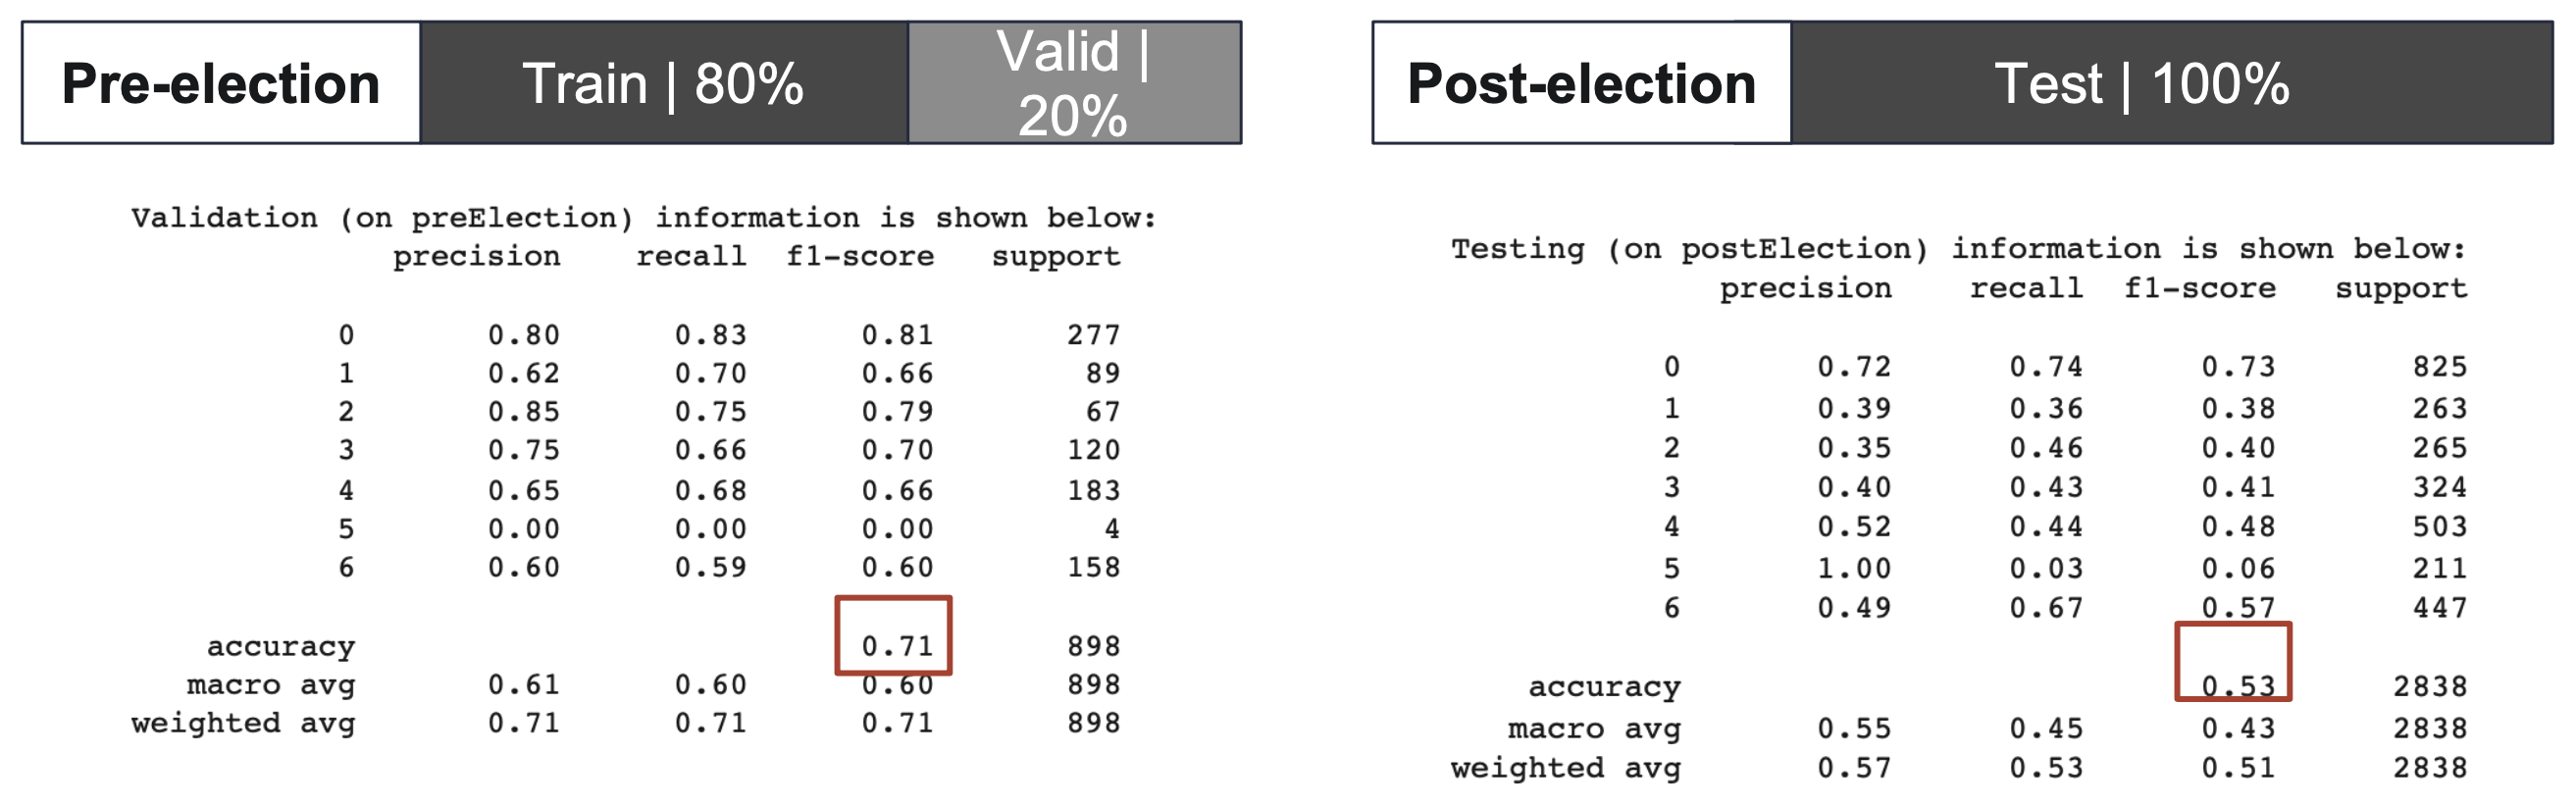
\includegraphics[width=\linewidth]{Figure/DNN.png}
    {\footnotesize 在驗證集時,模型分類
    的準確度可以達到0.71,而使用
    測試集測試時,分類的準確度則
    掉落至0.53。
    \par}
    \end{minipage}
    \caption{深層神經網絡分類模型的結果}
    \label{fig:DNN}
\end{figure*}
\begin{corollary}\label{cor:gap}
使用選前資料訓練的模型
無法準確地分類選後的資料,
說明選前選後,媒體的報導之間仍有
某些語意或報導主題的落差。
\end{corollary}

為了找出使選前選後媒體分類不準確的肇因,
我們萃取出選前與選後的語料中最常見
的幾項主題。
前後對照後發現,選前與選後的報導中,
僅有約$43\%$,不到一半的主題重疊。
舉例來說,選前常見的主題有「WuHan」、「Hong Kong」等,
而選後這些主題出現的頻率下降,
轉而「Taiwan」、「Biden」等主題
較多出現在報導內(見\cref{fig:topic})。
\begin{figure}[h!]
    \centering
    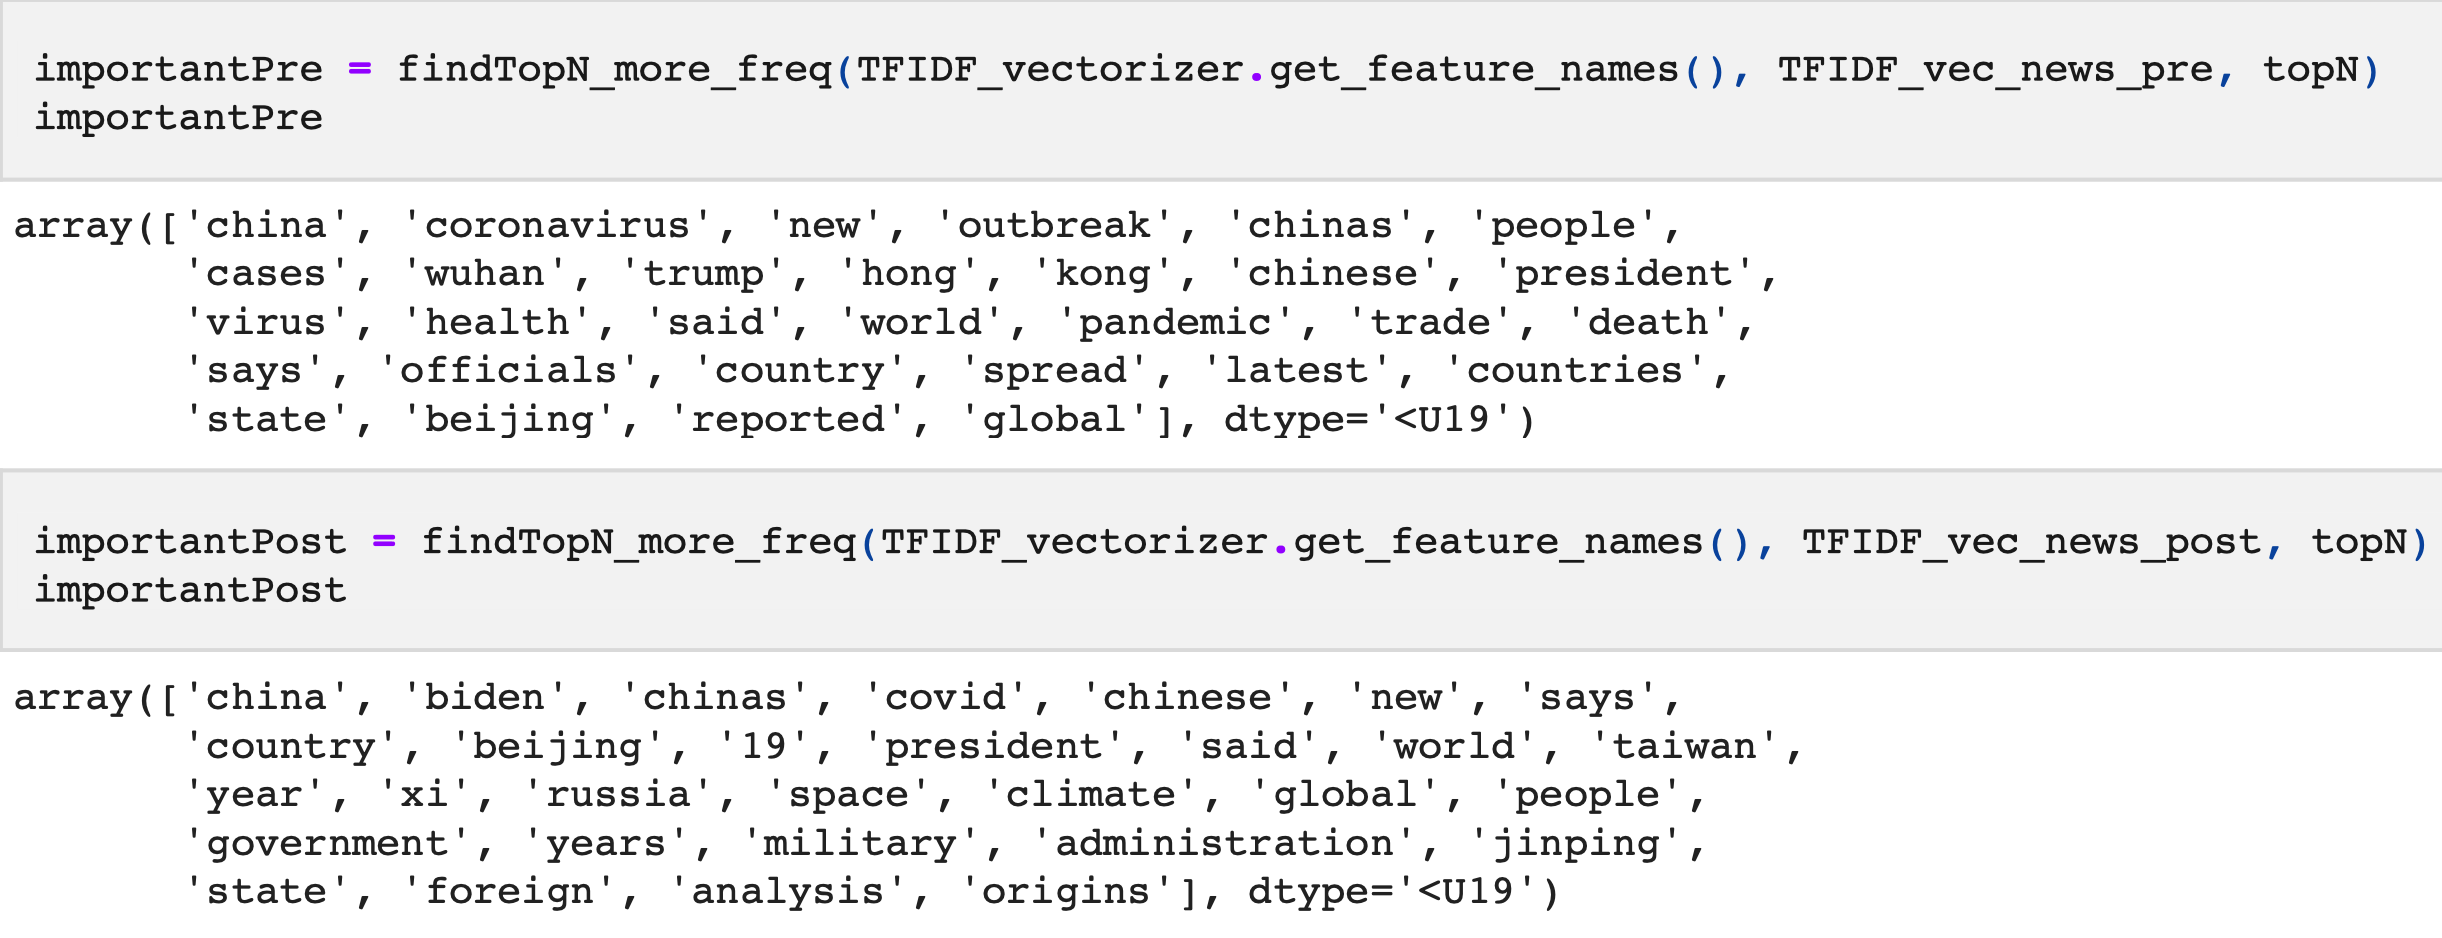
\includegraphics[width=1.0\linewidth]{Figure/freq.png}
    \caption{選舉前與選舉後常見的報導主題}
    \label{fig:topic}
\end{figure}


\begin{explain}\label{exp:gap}
由於選前選後資料的主題性重疊性太低,
因此就算使用深層神經網路,
訓練出來的模型依舊無法根據
媒體風格等準確分類選後的報導。
\end{explain}

自此,我們的實驗結果說明了
在選舉前與選舉後,媒體的報導行為
的確是有差異。

\section{結論}\label{sec:conclu}
本文的研究重點旨在探討美國總統候選人
對中態度的不同是否會影響選舉前後
美國媒體報導對中國的態度。
我們透過情感分析的模型計算出
媒體報導的情感分數,
並找出時間趨勢,證明選舉前後
美國媒體對中國的態度的確有所差異;
而我們也透過計算文本相似度、
萃取選舉前選舉後的報導主題異同等方法
說明了選舉前後美國媒體與中國有關的
報導主題並不相同。
基於我們研究的觀察,
未來可以繼續分析台灣選舉前後台灣媒體
對中國的態度是否與美國媒體
有類似的行為。

\bibliography{ref}
\end{document}
